% ----------------------------------------------------------
% VALIDAÇÕES DE SEGURANÇA, INTERFACE E CÓDIGO
% ----------------------------------------------------------
\section{Validações de segurança, interface e código}
Nessa seção são abordadas algumas validações que fizemos na nossa aplicação e a justificativa delas.

\subsection{Teste dos \textit{headers} da API}
Para os testes de \textit{headers} de segurança, foi usado o site \textit{\gls{secheaders}}, onde é possível verificar em qual nota se enquadrava a \ac{api} do projeto. Foram feitos testes de um dos nossos \textit{\glspl{endpoint}} (O resultado é o mesmo para todos), e durante o primeiro teste, o site indicou que nota F, pela resposta da aplicação não conter nenhum \textit{header} de segurança, então com base nesse resultado, foram adicionadas as dependências que faltavam e assim, foi possível subir a nota, como demonstra a \autoref{sec-headers}.

\begin{figure}[H]
	\centering
	\caption{\label{sec-headers}Validação dos \textit{headers}}
	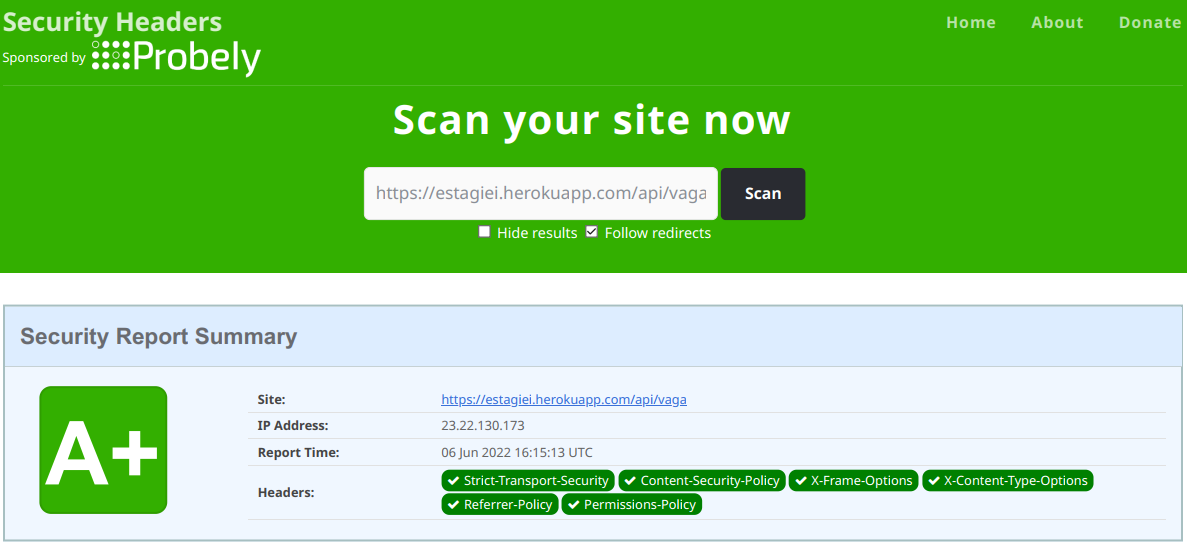
\includegraphics[width=0.95\textwidth]{../imagens/web-tests/grade-security-headers.png}
	\fonte{Os Autores.}
\end{figure}

\begin{figure}[htb]
	\caption{\label{qr-url-swagger}URL da documentação dos nossos \textit{\glspl{endpoint}} (\textit{Swagger UI})}
	\begin{center}
		\geraQRCode{https://estagiei.herokuapp.com/api/swagger-ui/}
		\legend{\url{https://estagiei.herokuapp.com/api/swagger-ui/}}
		\fonte{Os Autores.}
	\end{center}
\end{figure}

\subsection{Teste de \ac{tls} do \textit{\gls{frontend}}}
O sistema \emph{EstagiEI} também foi testado com relação ao certificado \ac{tls}, que indica se um site utiliza o protocolo \ac{https} ou não. Devido a aplicação estar hospedada no \textit{\gls{netlify}}, ele automaticamente já providencia um certificado com o \textit{\gls{letsencrypt}} quando é criado um domínio personalizado. Assim como mostra a \autoref{grade-server-test}, a aplicação possui um certificado \ac{tls} ativo.

\begin{figure}[H]
	\centering
	\caption{\label{grade-server-test}Teste de \ac{tls}}
	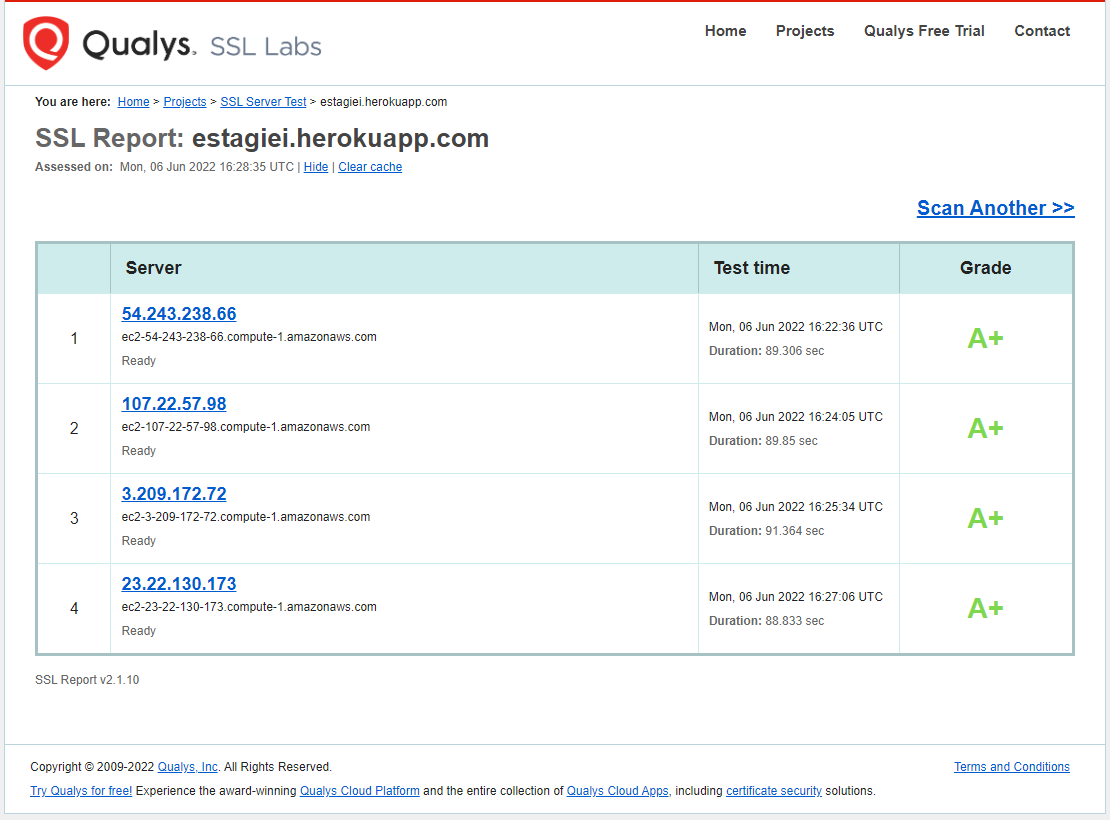
\includegraphics[width=0.95\textwidth]{../imagens/web-tests/grade-server-test.png}
	\fonte{Os Autores}
\end{figure}

\begin{figure}[htb]
	\caption{\label{qr-url-frontend}URL do \textit{\gls{frontend}} da nossa aplicação}
	\begin{center}
		\geraQRCode{https://estagiei.netlify.app/}
		\legend{\url{https://estagiei.netlify.app/}}
		\fonte{Os Autores.}
	\end{center}
\end{figure}

\subsection{Teste de desempenho do \textit{\gls{frontend}}}
Através da extensão \textit{\gls{lighthouse}}, foi verificado como estava o desempenho, acessibilidade, etc. Da tela de login, e foi percebido pontos a serem melhorados, principalmente na questão do desempenho. Pontos esses que serão ajustados no próximo semestre. A \autoref{lighthouse-test} ilustra o resultado.

\begin{figure}[H]
	\centering
	\caption{\label{lighthouse-test}Teste de desempenho do \textit{\gls{frontend}}}
	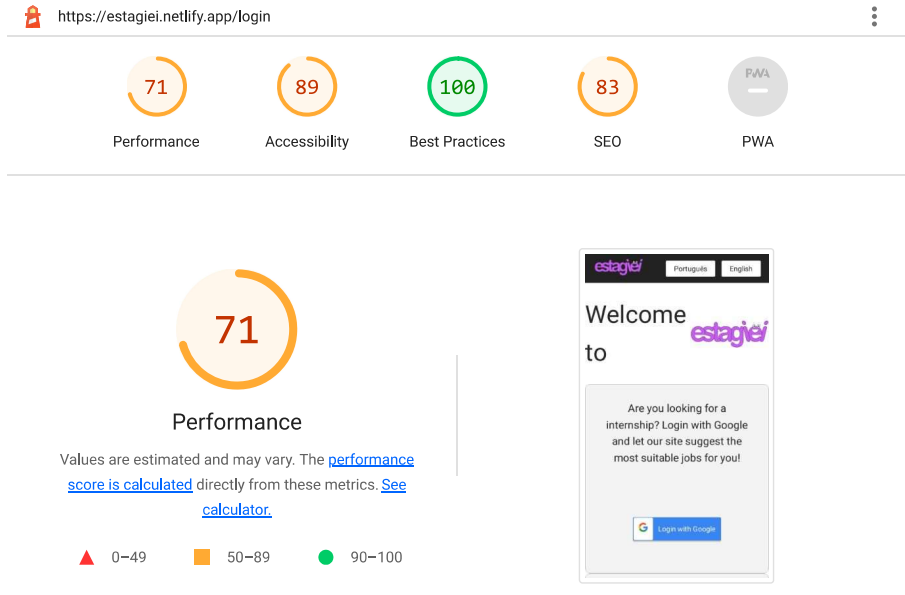
\includegraphics[width=0.95\textwidth]{../imagens/web-tests/lighthouse-test.png}
	\fonte{Os Autores.}
\end{figure}

\subsection{Análise de código}
Fizemos também uma verificação no nosso código, tanto no \textit{\gls{frontend}} como no \textit{\gls{backend}}, e o resultado foi relativamente satisfatório, faltando apenas alguns pontos que serão melhorados ao longo do tempo. As figuras \autoref{better-code-front} e \autoref{better-code-back} demonstram os resultados do \textit{\gls{frontend}} e \textit{\gls{backend}} respectivamente.

\begin{figure}[H]
	\centering
	\caption{\label{better-code-front}Análise de código do \textit{\gls{frontend}}}
	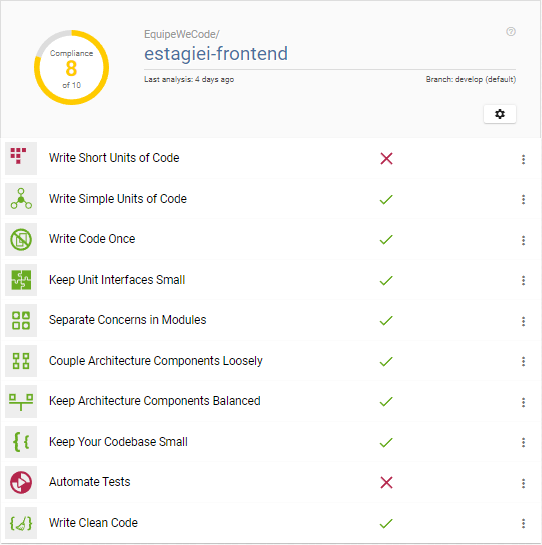
\includegraphics[width=0.95\textwidth]{../imagens/web-tests/better-code-front.png}
	\fonte{Os Autores.}
\end{figure}

\begin{figure}[H]
	\centering
	\caption{\label{better-code-back}Análise de código do \textit{\gls{backend}}}
	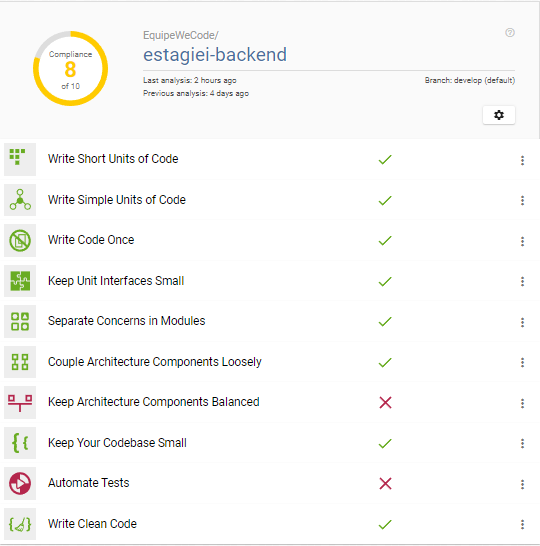
\includegraphics[width=0.95\textwidth]{../imagens/web-tests/better-code-back.png}
	\fonte{Os Autores.}
\end{figure}

\subsection{Validador \ac{html}}
Foi feito também uma verificação no \ac{html} do \textit{\gls{frontend}}. A \autoref{validador-html} demonstra o resultado.

\begin{figure}[H]
	\centering
	\caption{\label{validador-html}Validação do \ac{html}}
	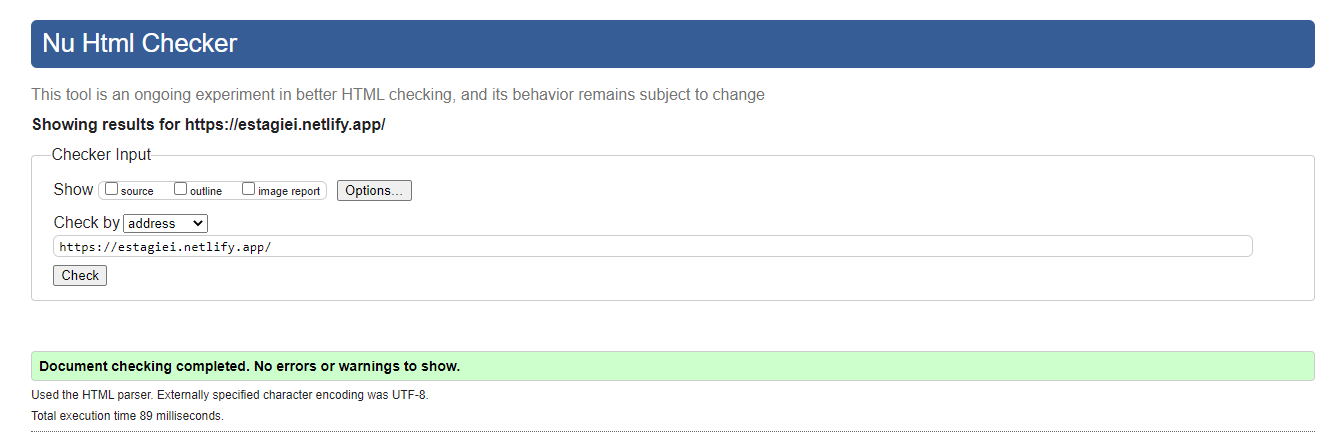
\includegraphics[width=0.95\textwidth]{../imagens/web-tests/validador-html.png}
	\fonte{Os Autores.}
\end{figure}